\documentclass[12pt]{article}
\usepackage[utf8]{inputenc}

\usepackage{graphicx}
\usepackage{tikz}
\usetikzlibrary{arrows}
\usepackage{booktabs}
\usepackage{tabularx}
\usepackage{lipsum}

\title{Different Negotiation Situations}
\author{Anna Fritz}
\date{August 2022}

\begin{document}

\begin{titlepage}
\maketitle
\end{titlepage}

Negotiation is the act of an \emph{appraiser} and \emph{target} agreeing on a protocol for attestation. 

\begin{figure}[hbtp]
    \centering 
    \input{negotiation-fig.tex}
    \caption[Negotiation process]{Negotiation protocol.}
    \label{fig:negotiation-fig}
  %%\description{Attestation sequence.}
  \end{figure}

\begin{table}
    \begin{tabularx}{\linewidth}{>{\parskip1ex}X@{\kern4\tabcolsep}>{\parskip1ex}X}
        \toprule
        \hfil\bfseries Pros
        &
        \hfil\bfseries Cons
        \\\cmidrule(r{3\tabcolsep}){1-1}\cmidrule(l{-\tabcolsep}){2-2}

        %% PROS, seperated by empty line or \par
        Gives appriser chance to understand target system and correctly formulate a request. \par
        Appraiser decides best protocol. \par
        Target ensures Appraiser is not aware of any protocols that expose sensitive information \par        
        &
        %% CONS, separated by empty line or \par
        More messages. This increases the network usage and is unfavorable to the IETF. \par 

        \\\bottomrule
    \end{tabularx}
    \caption{Pros and cons of 3 step negotiation}
\end{table}

\begin{figure}[hbtp]
    \centering 
    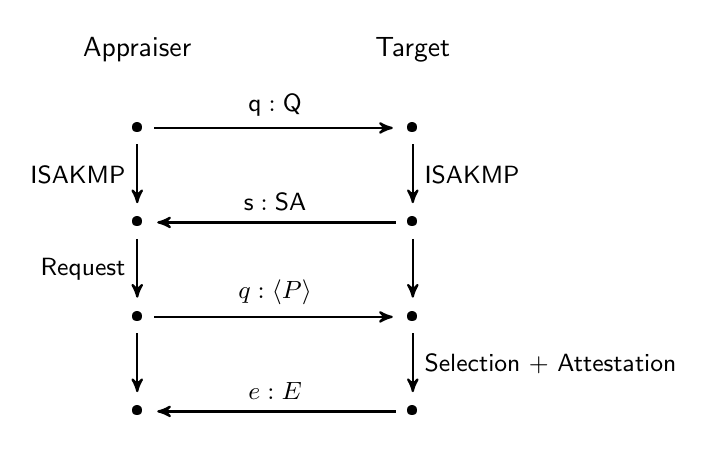
\begin{tikzpicture}[->,>=stealth',shorten >=1pt,auto,node distance=1.2cm,
    thick,main node/.style={rectangle,%%fill=blue!20,draw,
      font=\sffamily,minimum height=2mm,minimum width=2mm}]
  
  
    \node[main node] (RQ) {\textbullet};
    \node[main node] (SA) [below of=RQ] {\textbullet};
    \node[main node] (NM) [below of=SA] {\textbullet};
    \node[main node] (AM) [below of=NM] {\textbullet};
  %%  \node[main node] (CP) [below of=AM] {\textbullet};
  %%  \node[main node] (HW) [below of=CP] {\textbullet};
  %%  \node[main node] (AP) [below of=HW] {\textbullet};
  %%  \node[main node] (HWE) [node distance=3.5cm, right of=HW] {\textbullet};
  %%  \node[main node] (CPE) [node distance=3.5cm, right of=CP] {\textbullet};
    \node[main node] (AME) [node distance=3.5cm, right of=AM] {\textbullet};
    \node[main node] (NME) [node distance=3.5cm, right of=NM] {\textbullet};
    \node[main node] (SAE) [node distance=3.5cm, right of=SA] {\textbullet};  
    \node[main node] (RQE) [node distance=3.5cm, right of=RQ] {\textbullet};  
    \node[main node] (IN) [node distance=1.0cm, above of=RQ] {Appraiser};
    \node[main node] (OUT) [node distance=1.0cm, above of=RQE] {Target};
      
  
    \path[every node/.style={font=\sffamily\small, fill=white,inner sep=1pt}]
      (RQ) edge node[above=1mm] {$\mathsf{q:Q}$} (RQE)
      (SAE) edge node[above=1mm] {$\mathsf{s:SA}$} (SA)
      (NM) edge node[above=1mm] {$q:\langle P \rangle$} (NME)
      (AME) edge node[above=1mm] {$e:E$} (AM)
      %(CP) edge node[above=1mm] {$p:P$} (CPE)
      %(HWE) edge node[above=1mm] {$e:E$} (HW)
      (RQ) edge node[left=1mm] {ISAKMP} (SA)
      (RQE) edge node[right=1mm] {ISAKMP} (SAE)
      (SA) edge node[left=1mm] {Request} (NM)
      (SAE) edge node[right=1mm] {} (NME)
      (NM) edge node[left=1mm] {} (AM)
      (NME) edge node[right=1mm] {Selection + Attestation} (AME)
  %%    (AM) edge node[left=1mm] {Selection} (CP)
  %%    (AME) edge node[right=1mm] {} (CPE)
  %%    (CP) edge node[left=1mm] {} (HW)
  %%    (CPE) edge node[right=1mm] {Attestation} (HWE)
  %%    (HW) edge node[left=1mm] {Appraisal} (AP)
      ;
  \end{tikzpicture}
    \caption[Negotiation process]{Negotiation protocol.}
    \label{fig:negotiation-fig-2}
    %%\description{Attestation sequence.}
\end{figure}

\end{document}